

% --------------------------------------------------------------
\begin{frame}[fragile]
  \frametitle{Recent Progress}
  \begin{itemize}
    \item 1-D, 6 group neutronics model
    \item 1-D thermal hydraulics model
    \item Forward Difference Coupling 
    \item 3-D Mesh Development
  \end{itemize}
\end{frame}

% --------------------------------------------------------------
\begin{frame}[fragile]
  \frametitle{Coupled Kinetics}
  \footnotesize{
\begin{equation} 
  \frac{d}{dt}\left[
    \begin{array}{c}
      p\\
      \zeta_1\\
      .\\
      .\\
      .\\
      \zeta_J\\
      \omega_1\\
      .\\
      .\\
      .\\
      \omega_K\\
      T_{fuel}\\
      T_{cool}\\
      .\\
      .\\
      .\\
    \end{array}
    \right]
    =
    \left[
      \begin{array}{ c }
        \frac{\rho(t,T_{fuel},T_{cool},\cdots)-\beta}{\Lambda}p + 
        \displaystyle\sum^{j=J}_{j=1}\lambda_j\zeta_j\\
        \frac{\beta_1}{\Lambda} p - \lambda_1\zeta_1\\
        .\\
        .\\
        .\\
        \frac{\beta_J}{\Lambda}p-\lambda_J\zeta_J\\
        \kappa_1p - \lambda_1\omega_1\\
        .\\
        .\\
        .\\
        \kappa_{k} p - \lambda_k\omega_{k}\\
        f(p, C_p^{fuel}, T_{fuel}, T_{cool},\cdots)\\
        g(C_p^{cool}, T_{fuel}, T_{cool},\cdots)\\
        .\\
        .\\
        .\\
      \end{array}
      \right]
      \label{eqn:ourPRKE}
    \end{equation}
  
  }
\end{frame}

% --------------------------------------------------------------
\begin{frame}[fragile]
  \frametitle{Coupled Kinetics}
  \footnotesize{
\begin{equation} 
  \frac{d}{dt}\left[
    \begin{array}{c}
      p\\
      \zeta_1\\
      .\\
      .\\
      .\\
      \zeta_J\\
      \omega_1\\
      .\\
      .\\
      .\\
      \omega_K\\
      \textcolor{red}{T_{fuel}}\\
      \textcolor{red}{T_{cool}}\\
      .\\
      .\\
      .\\
    \end{array}
    \right]
    =
    \left[
      \begin{array}{ c }
        \frac{\textcolor{red}{\rho(t,T_{fuel},T_{cool},\cdots)}-\beta}{\Lambda}p + 
        \displaystyle\sum^{j=J}_{j=1}\lambda_j\zeta_j\\
        \frac{\beta_1}{\Lambda} p - \lambda_1\zeta_1\\
        .\\
        .\\
        .\\
        \frac{\beta_J}{\Lambda}p-\lambda_J\zeta_J\\
        \kappa_1p - \lambda_1\omega_1\\
        .\\
        .\\
        .\\
        \kappa_{k} p - \lambda_k\omega_{k}\\
        f(p, C_p^{fuel}, T_{fuel}, T_{cool},\cdots)\\
        g(C_p^{cool}, T_{fuel}, T_{cool},\cdots)\\
        .\\
        .\\
        .\\
      \end{array}
      \right]
      \label{eqn:note_rho_prke}
    \end{equation}
  
  }
\end{frame}



% --------------------------------------------------------------
\begin{frame}[fragile]
  \frametitle{Neutronics Block}
  \footnotesize{
\begin{equation} 
  \frac{d}{dt}\left[
    \begin{array}{c}
      p\\
      \zeta_1\\
      .\\
      .\\
      .\\
      \zeta_J\\
      \omega_1\\
      .\\
      .\\
      .\\
      \omega_K\\
    \end{array}
    \right]
    =
    \left[
      \begin{array}{ c }
        \frac{\rho(t,T_{fuel},T_{cool},\cdots)-\beta}{\Lambda}p + 
        \displaystyle\sum^{j=J}_{j=1}\lambda_j\zeta_j\\
        \frac{\beta_1}{\Lambda} p - \lambda_1\zeta_1\\
        .\\
        .\\
        .\\
        \frac{\beta_J}{\Lambda}p-\lambda_J\zeta_J\\
        \kappa_1p - \lambda_1\omega_1\\
        .\\
        .\\
        .\\
        \kappa_{k}p - \lambda_k\omega_{k}\\
      \end{array}
      \right]
      \label{eqn:neutronics_prke}
    \end{equation}
  
  }
\end{frame}

% --------------------------------------------------------------
\begin{frame}[fragile]
  \frametitle{Neutronics Data Needs}
\footnotesize{
  \begin{align}
    \rho(t,&T_{fuel},T_{cool},T_{mod}, T_{refl}) = \mbox{ reactivity, [pcm]}\\
    \beta &= \mbox{ fraction of neutrons that are delayed}\\ 
    \beta_j &= \mbox{ fraction of delayed neutrons from precursor group j}\\  
    \zeta_j &= \mbox{ concentration of precursors of group j}\\ 
    \lambda^{d}_j &= \mbox{ decay constant of precursor group j}\\ 
    \Lambda &= \mbox{ mean generation time ? }\\
    \omega_k &= \mbox{ decay heat from FP group k}\\ 
    \kappa_k &= \mbox{ heat per fission for decay FP group k}\\ 
    \lambda^{FP}_k &= \mbox{ decay constant for decay FP group k} 
  \end{align}
}

\end{frame}
% --------------------------------------------------------------
\begin{frame}[fragile]
  \frametitle{Neutronics : Delayed Neutron Model}

    \begin{table}
      \begin{tabular}{|l|c|c|c|c|}
        \hline
        j & $t_{1/2}$ & $\lambda^d_j$  & $\eta_j$ & $\beta_j$\\
          &   $[s]$   &    $[1/s]$     & $[n/f]$  & \\
        \hline
        1   &  $ 55.72 $  &  $ 0.0124 $  &  $ 0.00052 $  &  $ 0.000215$  \\
        2   &  $ 22.72 $  &  $ 0.0305 $  &  $ 0.00546 $  &  $ 0.001424$  \\
        3   &  $ 6.22  $  &  $ 0.111  $  &  $ 0.00310 $  &  $ 0.001274$  \\
        4   &  $ 2.30  $  &  $ 0.301  $  &  $ 0.00624 $  &  $ 0.002568$  \\
        5   &  $ 0.614 $  &  $ 1.14   $  &  $ 0.00182 $  &  $ 0.000748$  \\
        6   &  $ 0.230 $  &  $ 3.01   $  &  $ 0.00066 $  &  $ 0.000273$  \\
        \hline
      \end{tabular}
      \caption{Delayed neutron data Decay heat data, $^{235}$U thermal fission. 
    Lamarsh.}
      \label{tab:delayedneutrons}
    \end{table}

\end{frame}

% --------------------------------------------------------------
\begin{frame}[fragile]
  \frametitle{Neutronics : Decay Heat Model}
    \begin{table}
      \begin{tabular}{|l|c|c|}
        \hline
        k & $\lambda^{FP_k}$ & $\kappa_k$\\
                          &  $[1/s]$         & $[MeV/fission-s]$ \\
        \hline
        1   &  $ 6.587\times10^{  0} $  &  $ 2.658\times10^{  0}$ \\
        2   &  $ 1.490\times10^{ -1} $  &  $ 4.619\times10^{ -1}$ \\
        3   &  $ 2.730\times10^{ -1} $  &  $ 6.069\times10^{ -2}$ \\
        4   &  $ 2.173\times10^{ -2} $  &  $ 5.593\times10^{ -3}$ \\
        5   &  $ 1.961\times10^{ -3} $  &  $ 6.872\times10^{ -4}$ \\
        6   &  $ 1.025\times10^{ -4} $  &  $ 6.734\times10^{ -5}$ \\
        7   &  $ 4.923\times10^{ -6} $  &  $ 6.413\times10^{ -6}$ \\
        8   &  $ 2.679\times10^{ -7} $  &  $ 6.155\times10^{ -7}$ \\
        9   &  $ 1.452\times10^{ -8} $  &  $ 8.288\times10^{ -8}$ \\
       10   &  $ 1.893\times10^{ -9} $  &  $ 1.923\times10^{ -8}$ \\
       11   &  $ 1.633\times10^{-10} $  &  $ 1.214\times10^{ -9}$ \\
       \hline
      \end{tabular}
      \caption{Decay heat data, ANS/ANSI 5.1-1971 for $^{235}$U thermal fission.}
      \label{tab:decayheat}
    \end{table}

\end{frame}

% --------------------------------------------------------------

\begin{frame}[fragile]
  \frametitle{Neutronics : Reactivity Coefficients}
    \begin{table}
      \begin{tabular}{|l|c|c|c|}
        \hline
        Component & $T_{0}$  &  $T_0$ & $\frac{\partial\alpha}{\partial T}$\\
                  & $[K]$    &  $[K]$ & $[pcm/K]$ \\
        \hline
        fuel  & 730 & 1003.15 & -3.8 \\
        cool  & 650 &  923.15 & -1.8 \\
        mod   & 700 &  973.15 & -0.7 \\
        refl  & 650 &  923.15 &  \textcolor{red}{1.8} \\
        \hline
      \end{tabular}
      \caption{Temperature coefficients of reactivity for the PB-FHR Mk1. 
      Cisneros.}
      \label{tab:decayheat}
    \end{table}

\end{frame}

% --------------------------------------------------------------

\begin{frame}[fragile]
  \frametitle{Neutronics : Reactivity Insertion Model}
  \begin{align}
    \rho_{ext} &= \left\{
                  \begin{array}{l}
                            0 \\
                            \mbox{ ramp } \\
                            \mbox{ pulse } \\
                            \mbox{ prompt jump }\\
                            \mbox{ control rod drop }\\
                            \mbox{ . } \\
                            \mbox{ . } \\
                            \mbox{ . } \\
                  \end{array}
                  \right.
  \end{align}
\end{frame}

% --------------------------------------------------------------
\begin{frame}[fragile]
  \frametitle{Thermal Hydraulics Block}
  \footnotesize{
  \begin{equation} 
  \frac{d}{dt}\left[
    \begin{array}{c}
      T_{fuel}\\
      T_{cool}\\
      .\\
      .\\
      .\\
    \end{array}
    \right]
    =
    \left[
      \begin{array}{ c }
        f(p, C_p^{fuel}, T_{fuel}, T_{cool},\cdots)\\
        g(C_p^{cool}, T_{fuel}, T_{cool},\cdots)\\
        .\\
        .\\
        .\\
      \end{array}
      \right]
      \label{eqn:th_prke}
    \end{equation}
  
  }
\end{frame}



% --------------------------------------------------------------
\begin{frame}[fragile]
  \frametitle{Thermal Hydraulics Block}
  \footnotesize{
  \begin{equation} 
  \frac{d}{dt}\left[
    \begin{array}{c}
      T_{fuel} \\
      T_{cool} \\
      T_{mod} \\
      T_{refl} \\
    \end{array}
    \right]
    =
    \left[
      \begin{array}{ r }
        f(p, C_p^{fuel}, \rho_{fuel}, T_{fuel}, C_p^{cool}, v_{cool}, T_{cool},\\ 
          C_p^{mod}, T_{mod}, A_{fuel}, A_{mod}, \cdots )\\
          \\
        g(C_p^{fuel}, \rho_{fuel}, T_{fuel}, C_p^{cool}, v_{cool}, \rho_{cool},\\
          T_{cool}, A_{fuel}, \cdots )\\
          \\
        m(C_p^{fuel}, \rho_{fuel}, T_{fuel}, C_p^{cool}, v_{cool}, \rho_{cool},T_{cool},\\
         C_p^{mod}, \rho_{mod}, T_{mod}, A_{fuel}, A_{mod}, \cdots )\\
        \\
        r(C_p^{fuel}, \rho_{fuel}, T_{fuel}, C_p^{cool}, v_{cool}, \rho_{cool}, T_{cool},\\
         C_p^{mod}, \rho_{mod}, T_{mod}, A_{fuel}, A_{mod}, \cdots )\\
      \end{array}
      \right]
      \label{eqn:th_prke_fuller}
    \end{equation}
  
  }
\end{frame}


% --------------------------------------------------------------

\begin{frame}[fragile]
  \frametitle{Thermal Hydraulics Data Needs}
\footnotesize{
  \begin{align} 
    \rho_{c} &= \mbox{ density, for each component c [$kg/m^3$]}\\
    c_{p,c} &= \mbox{ specific heat capacity, for each component c [$J/m-K$]}\\
    k_{c} &= \mbox{ thermal conductivity, for each component c [$J/m-K$]}\\
    R_{th,c} &= \mbox{ thermal resistivity, for each component c }\\
    . &\\\nonumber
    . &\\\nonumber
    . &\nonumber
  \end{align}
}
\end{frame}
% --------------------------------------------------------------


\begin{frame}[fragile]
  \frametitle{Thermal Hydraulics : Heat Transfer Models }
\footnotesize{
  \begin{align} 
    \frac{dT_{fuel}}{dt} &=  - |cond|_{cool} - |cond|_{mod} - |conv|_{cool} + |fission|\\
    \frac{dT_{cool}}{dt} &=  + |cond|_{fuel} - |conv|_{cool} - |conv|_{refl} \\
    \frac{dT_{mod}}{dt}  &=  + |cond|_{fuel}\\
    \frac{dT_{refl}}{dt} &=  + |cond|_{cool}
  \end{align}
}
\end{frame}

% --------------------------------------------------------------
\begin{frame}[fragile]
  \frametitle{Coupling : Operator Splitting}
  Here, we treat neutronics and thermal hydraulics separately at 
  each time step with \textbf{forward Euler}. The values for $T_{fuel}$, 
  $T_{cool}$, $T_{mod}$, and $T_{refl}$ at time $t_n$ 
  are passed between physics subblocks, and the process is repeated.
  \footnotesize{
  \begin{align} 
    U^n &= \left[
                  \begin{array}{ c }
                    N^n\\
                    T^n\\
                  \end{array}
                  \right]\\
    N^{n+1} &= N^n + kf(U^n)\\
    \nonumber\\
    U^* &= \left[
                  \begin{array}{ c }
                    N^{n+1}\\
                    T^n\\
                  \end{array}
                  \right]\\
    T^{n+1} &= T^n + kf(U^*)
  \end{align}
  }
\end{frame}

% --------------------------------------------------------------
\begin{frame}[fragile]
  \frametitle{Coupling : Explicit Method Stability}
  \begin{figure}[htbp!]
    \begin{center}
      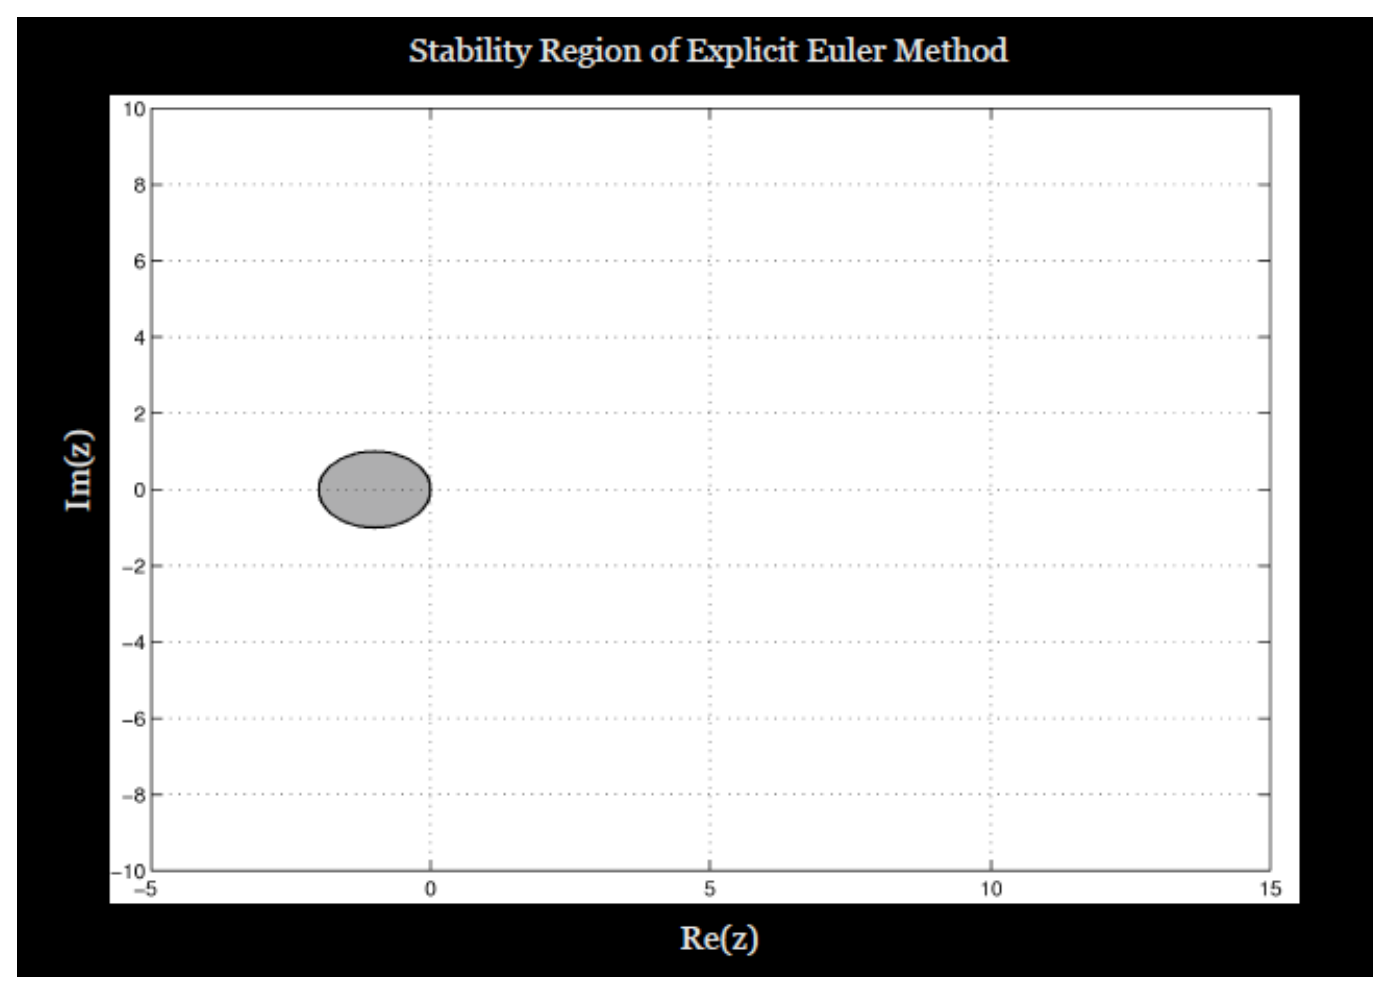
\includegraphics[width=0.8\textwidth]{./progress/euler.eps}
    \end{center}
    \caption{In addition to the loss of nonlinear residuals in the operator 
    splitting technique, the small stability region of explicit Runge-Kutta methods is 
  a drawback.}
    \label{fig:euler_stability}
  \end{figure}

\end{frame}

% --------------------------------------------------------------
\begin{frame}[fragile]
  \frametitle{Coupling : Implicit Method Stability}
  \begin{figure}[htbp!]
    \begin{center}
      \includegraphics[width=0.8\textwidth]{./progress/radau.eps}
    \end{center}
    \caption{Implicit Runge-Kutta methods, however, can be more stable. RadauII-5, for example, has a large stability region.}
    \label{fig:radau_stability}
  \end{figure}

\end{frame}


% --------------------------------------------------------------
\begin{frame}[fragile]
  \frametitle{Coupling : Jacobian}
BUT, recasting the whole problem into a Newton's solve for implicit Runge-Kutta
requires calculation of the Jacobian matrix. Direct computation of the (22x22)
Jacobian is inherently complex. 

However, Jacobian Free Newton-Krylov solves this. So, MOOSE will be used for
the implicit effort.

\end{frame}


% --------------------------------------------------------------
\begin{frame}[fragile]
  \frametitle{Coupling : MOOSE}
  One of the first steps to using MOOSE is building a mesh.
\end{frame}

